\appendix
\renewcommand{\thesection}{\textbf{Appendix \Alph{section}}}

\section{Sample Calcs} \label{apx:sample_calc}
\begin{enumerate}[wide,label=\textbf{\arabic*}., labelindent=0pt]

    \item \textbf{Wing Loading}
        \[W/S = \frac{W}{S_{ref}}\]
        $ W =$ weight [oz]\\
        $S_{ref} =$ wing reference area [ft$^2$]\\
        
        \begin{align*}
            W/S &= \frac{47.867}{16985}\\
            &= 9.18 \text{ oz/ft$^2$}\\
        \end{align*}
        
        \item \textbf{Aspect Ratio}
        \[AR = \frac{b^2}{S_{ref}}\]
        $ b =$ span [in]\\
        $S_{ref} =$ wing reference area [in$^2$]\\
        
        \begin{align*}
            AR &= \frac{69.8^2}{746.330}\\
            &= 6.530 \text{ N.D.}\\
        \end{align*}
    
    \item \textbf{Center of Gravity}
        \[x_{cg} = \frac{\sum_i m_i x_i }{\sum_i m_i}\]
        $ m_i =$ mass of component [g]\\
        $ x_i =$ distance from tip in x-direction of component [in]\\
    
        
        \begin{align*}
            \sum_i m_i &= (32)+(220)+(41)+(36.6)+(8)+(72)+(39.4)+(776)+(162) = 1387\\
            x_{cg} &= \frac{(32)(0)}{(1387)} + \frac{(220)(56.3)}{(1387)} + \frac{(41)(99.2)}{(1387)} + \frac{(36.6)(149.9)}{(1387)} + \frac{(8)(179.9)}{(1387)} + \frac{(72)(297.5)}{(1387)} \\
            &+ \frac{(39.4)(269.9)}{(1387)} + \frac{(776)(295)}{(1387)} + \frac{(162)(355)}{(1387)} = 244.6 mm\\
        \end{align*}
        
    \item \textbf{Taper Ratio}
        \[\lambda = \frac{c_t}{c_r}\]
        $ c_t =$ tip chord [in]\\
        $ c_r =$ root chord [in]\\
        
        \begin{align*}
            \lambda &= \frac{7.5}{14.5}\\
            &= 0.517 \text{ N.D.}\\
        \end{align*}
        
    \item \textbf{Power to Weight Ratio}
        \[P/W = \frac{P}{W}\]
        $ P =$ power [W]\\
        $ W =$ weight [g]\\
        
        \begin{align*}
            P/W &= \frac{266.4}{1357}\\
            &= 0.196 \text{ W/g}\\
        \end{align*}
 
\section{Engineering Drawings} \label{apx:eng_drawings}
    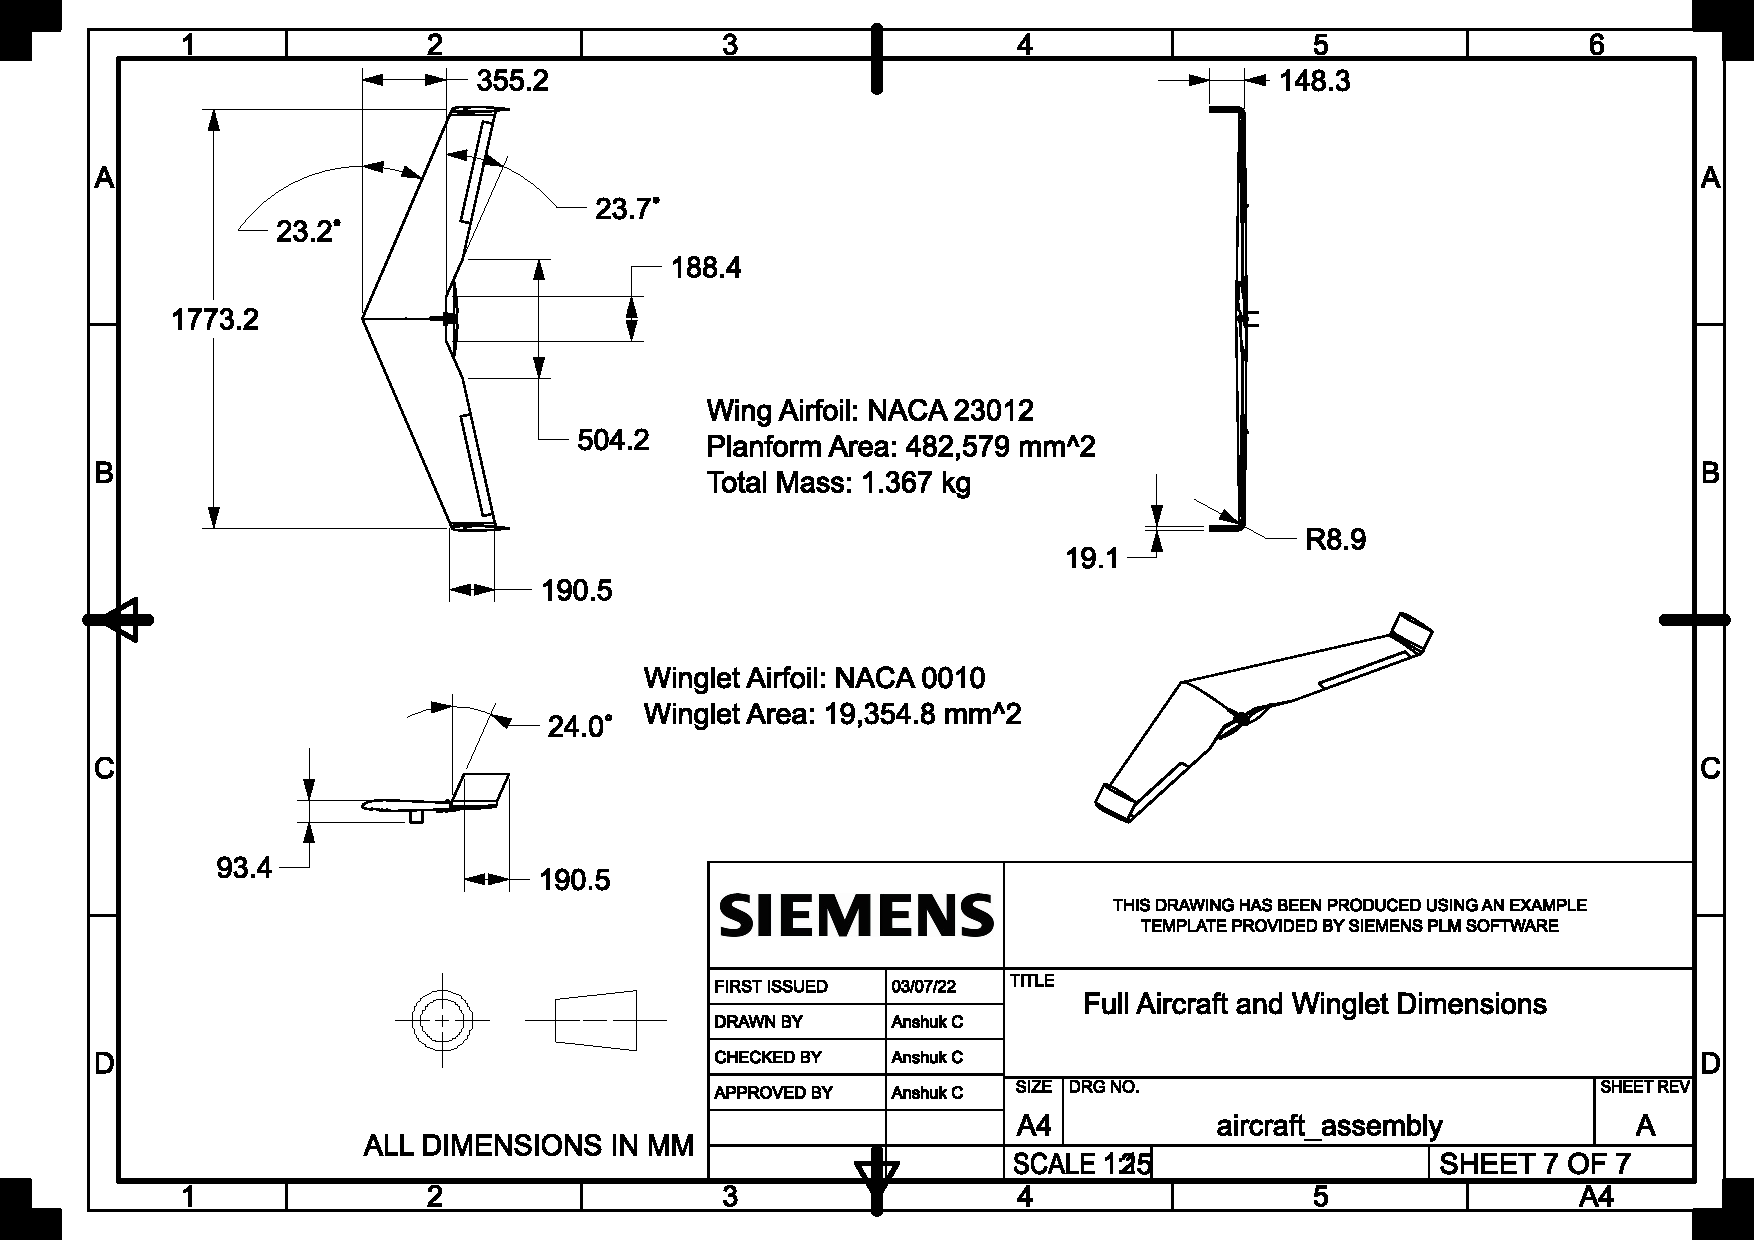
\includepdf[pages=-,angle=90]{homeworks/homework4/report/Figure/anshukc2_aircraft_dimensions.pdf}
    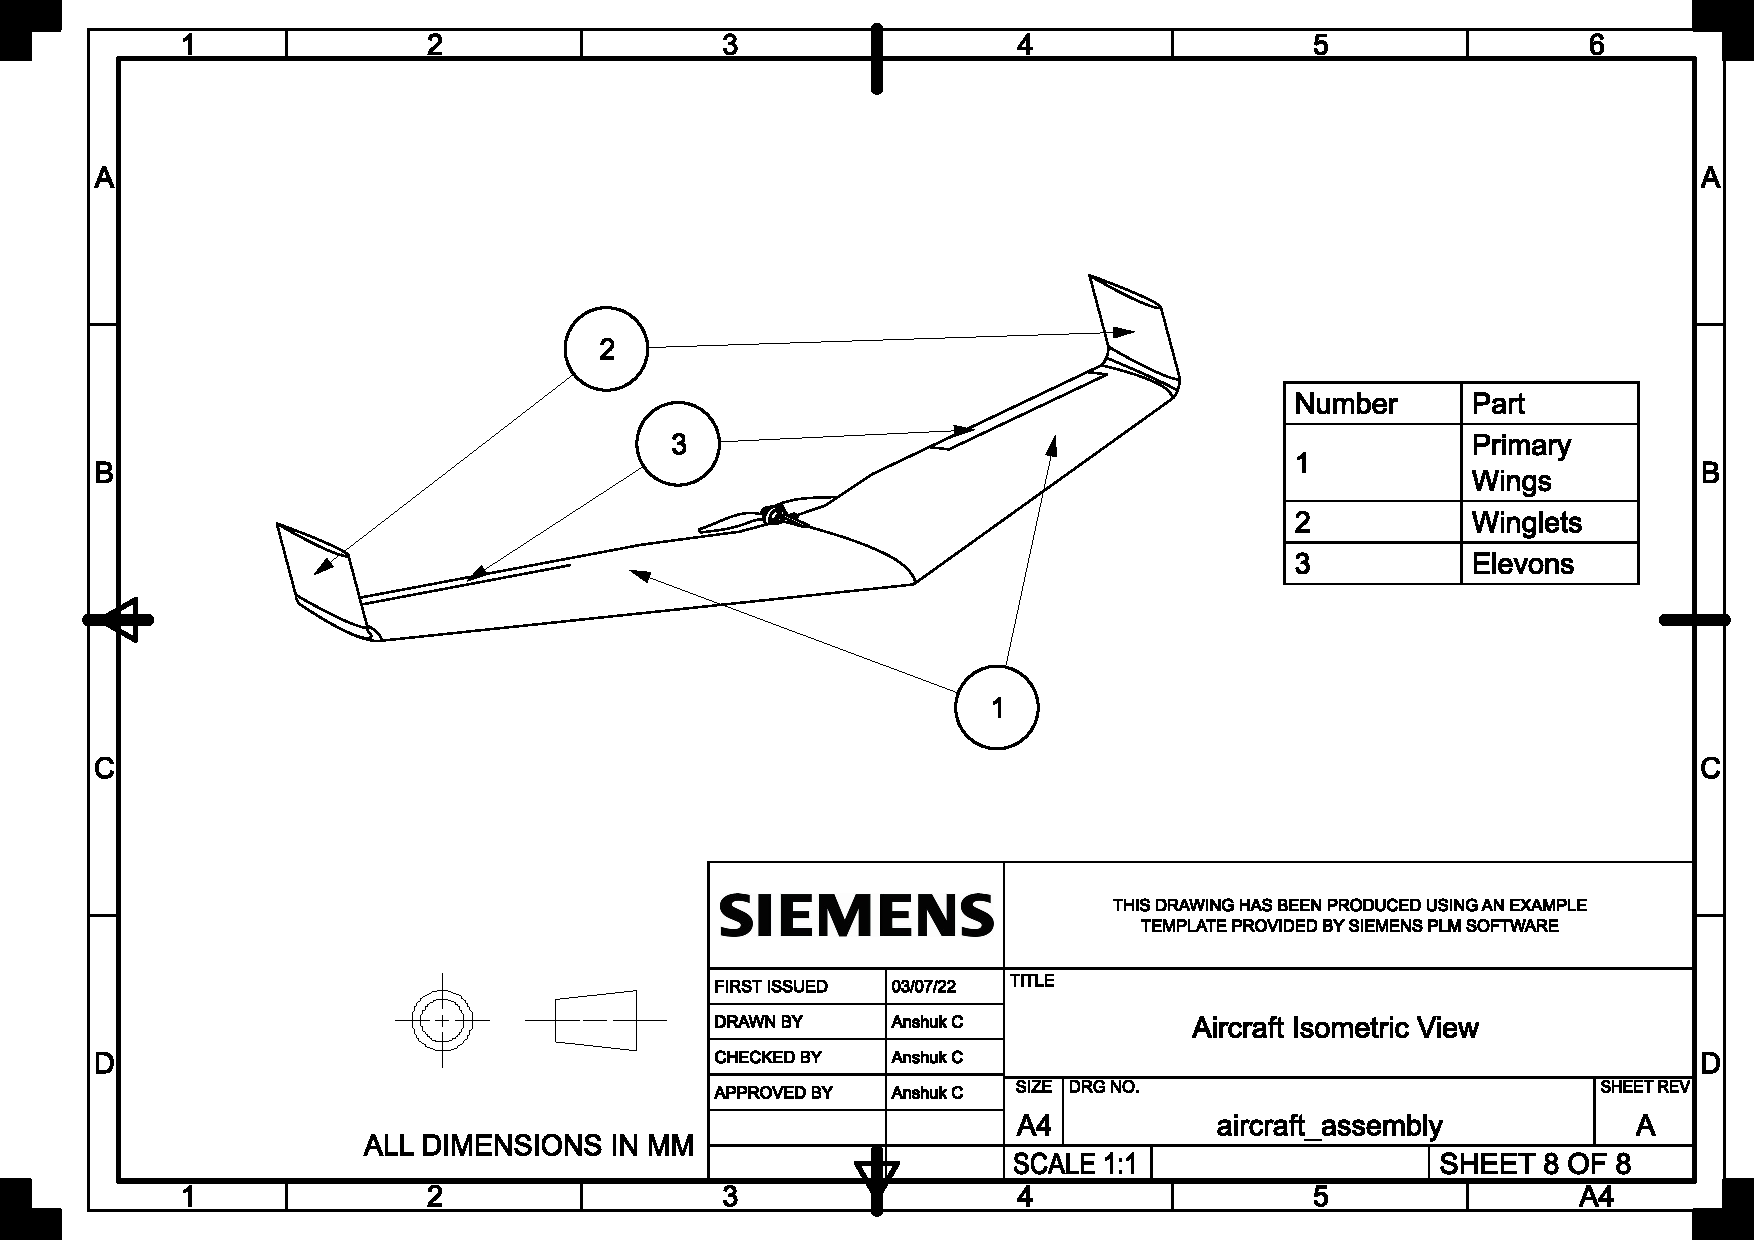
\includepdf[pages=-,angle=90]{homeworks/homework4/report/Figure/anshukc2_aircraft_isometric_drawing.pdf}
    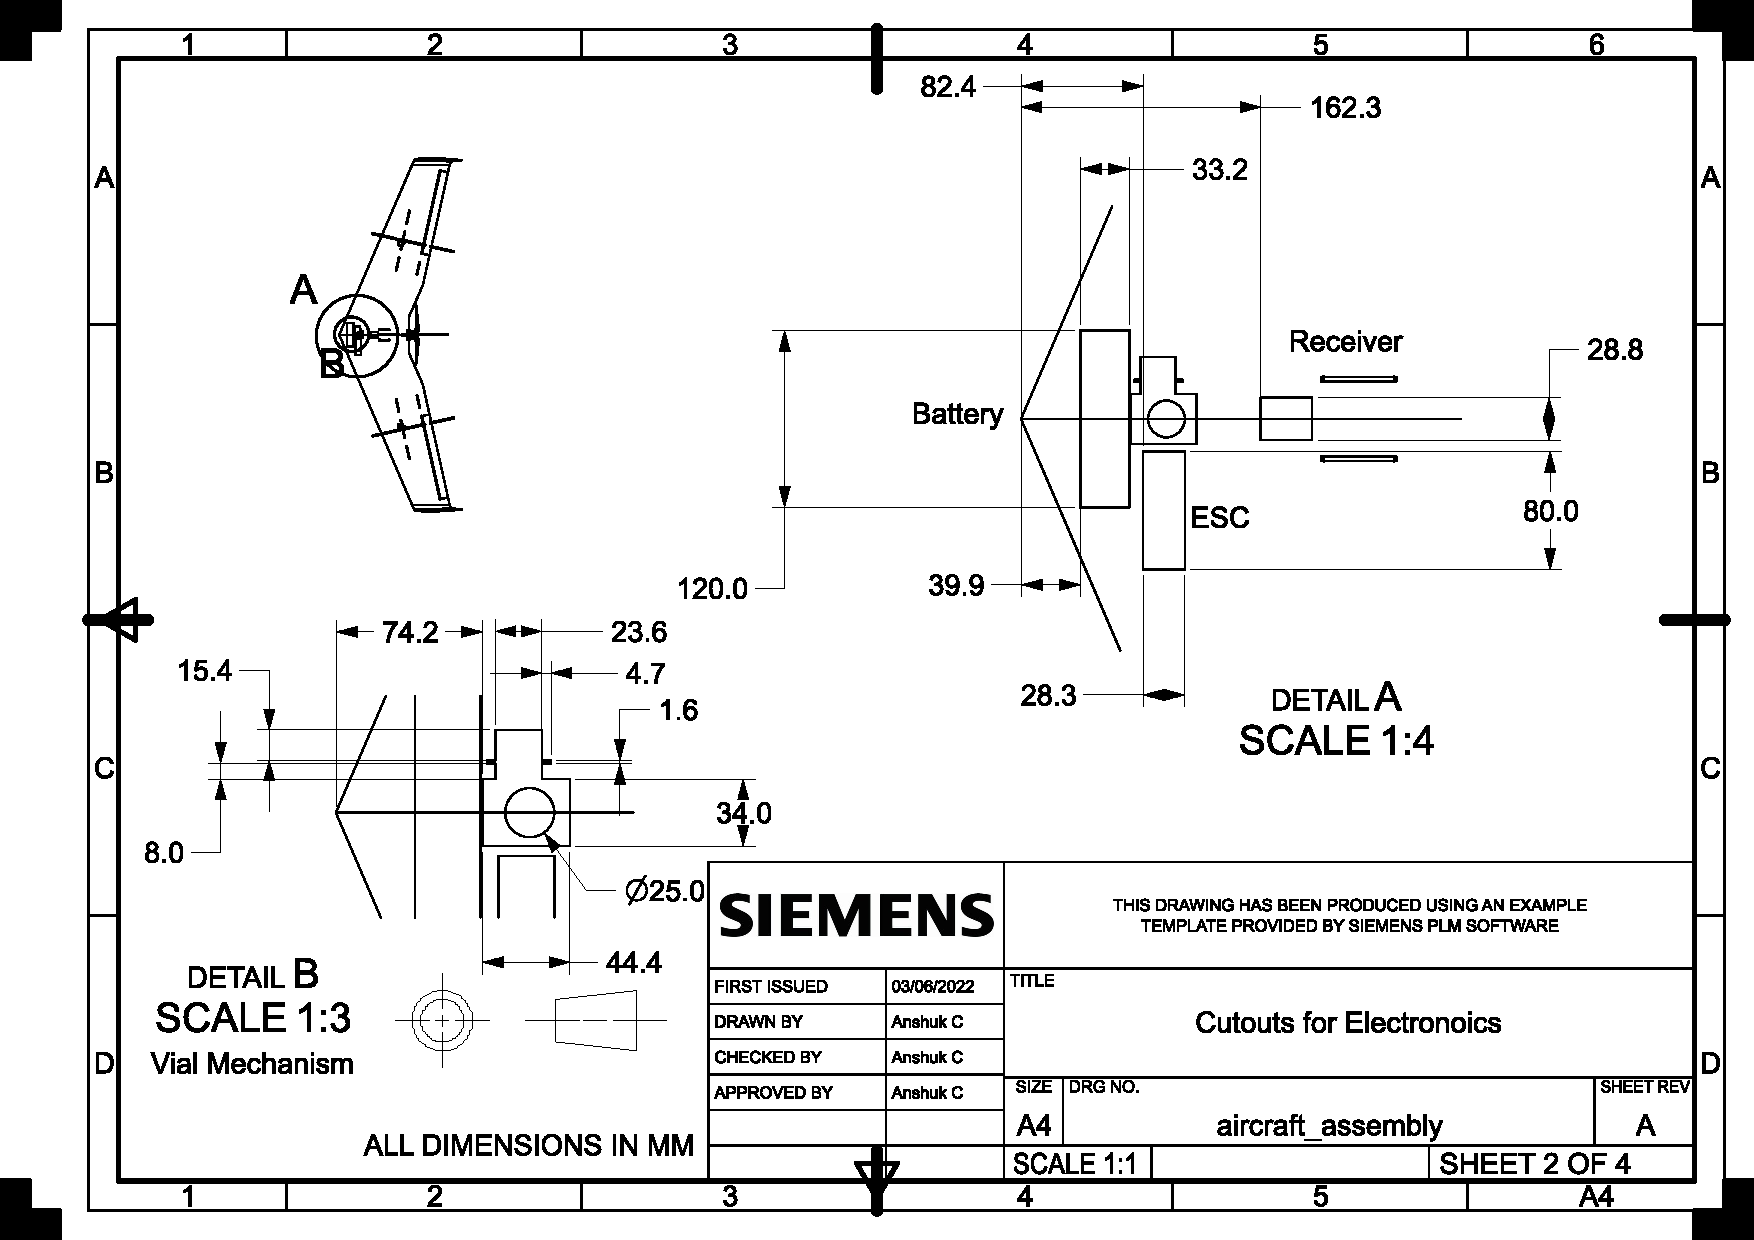
\includepdf[pages=-,angle=90]{homeworks/homework4/report/Figure/electronics_cutouts.pdf}
    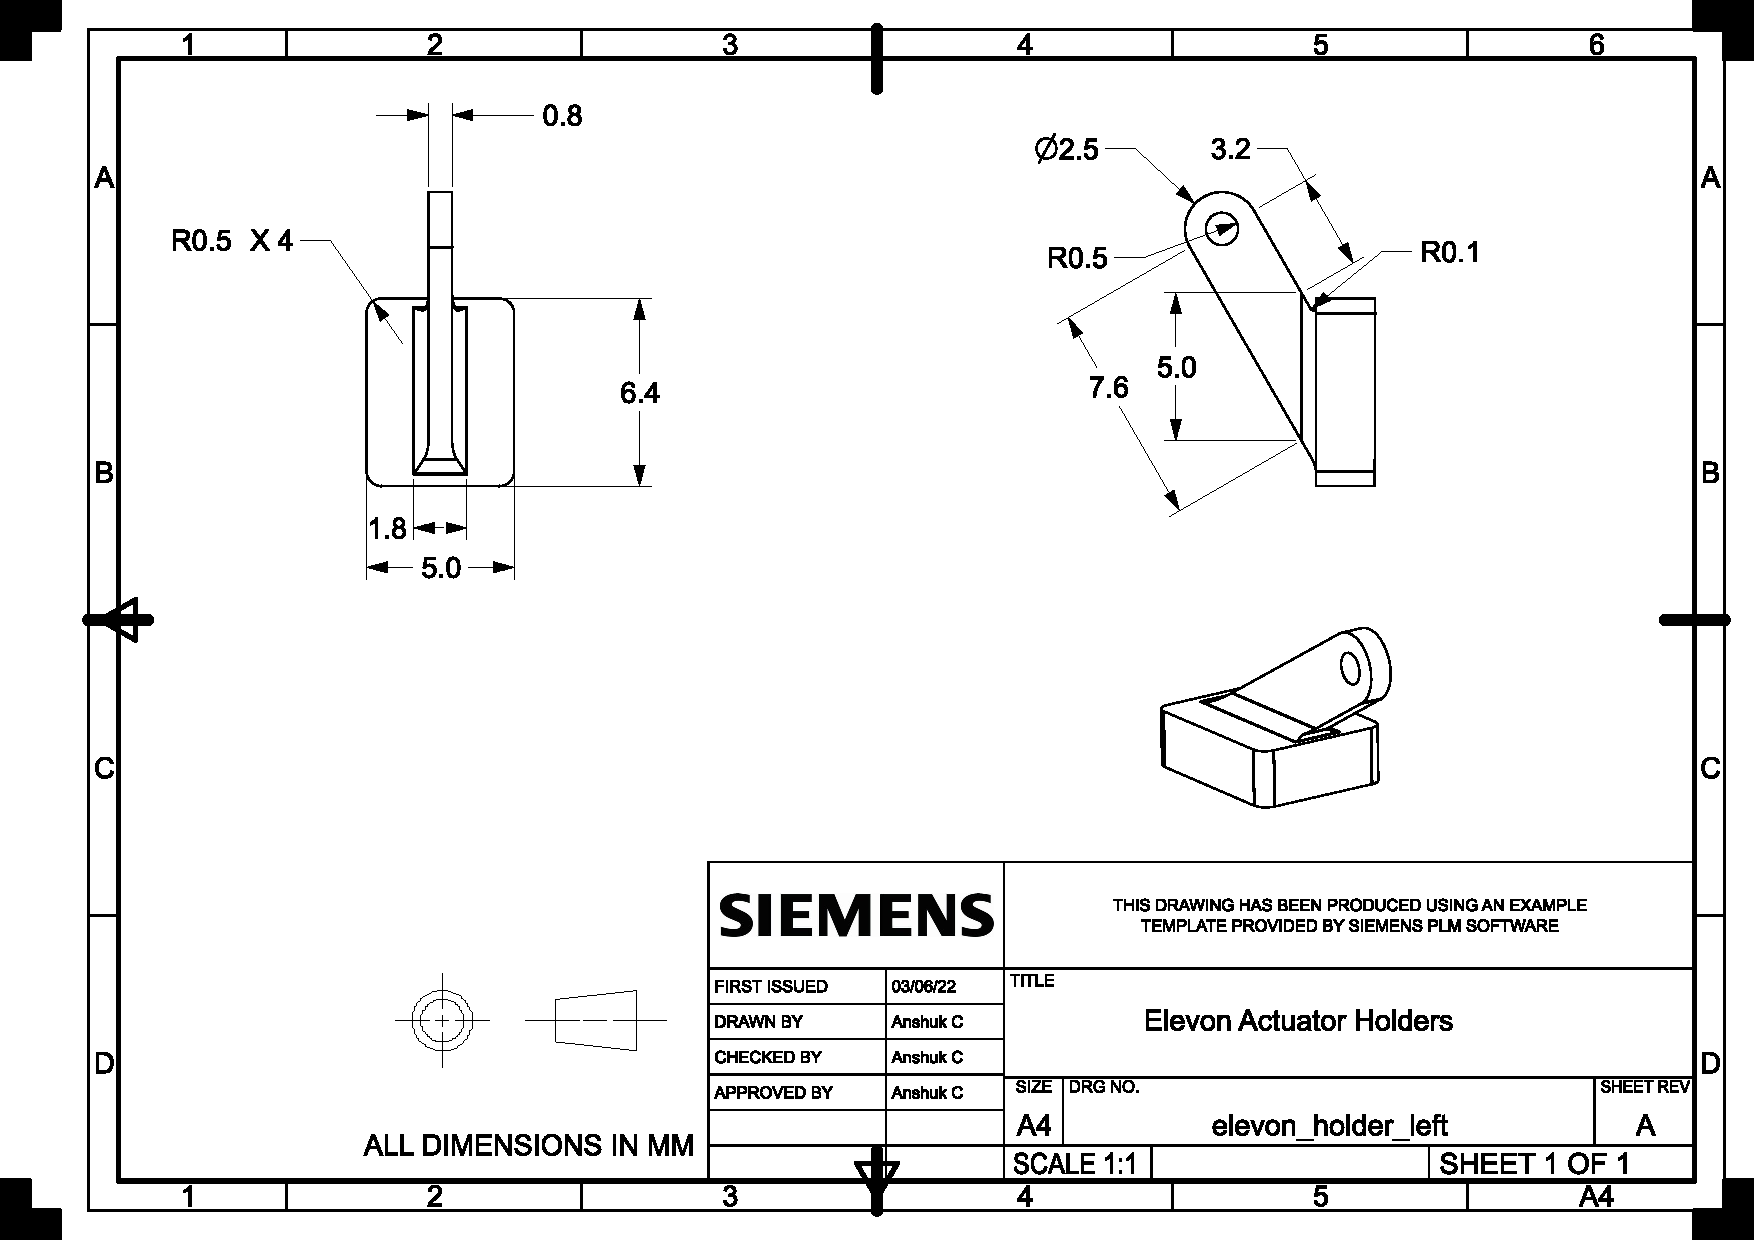
\includepdf[pages=-,angle=90]{homeworks/homework4/report/Figure/elevon_holders.pdf}
    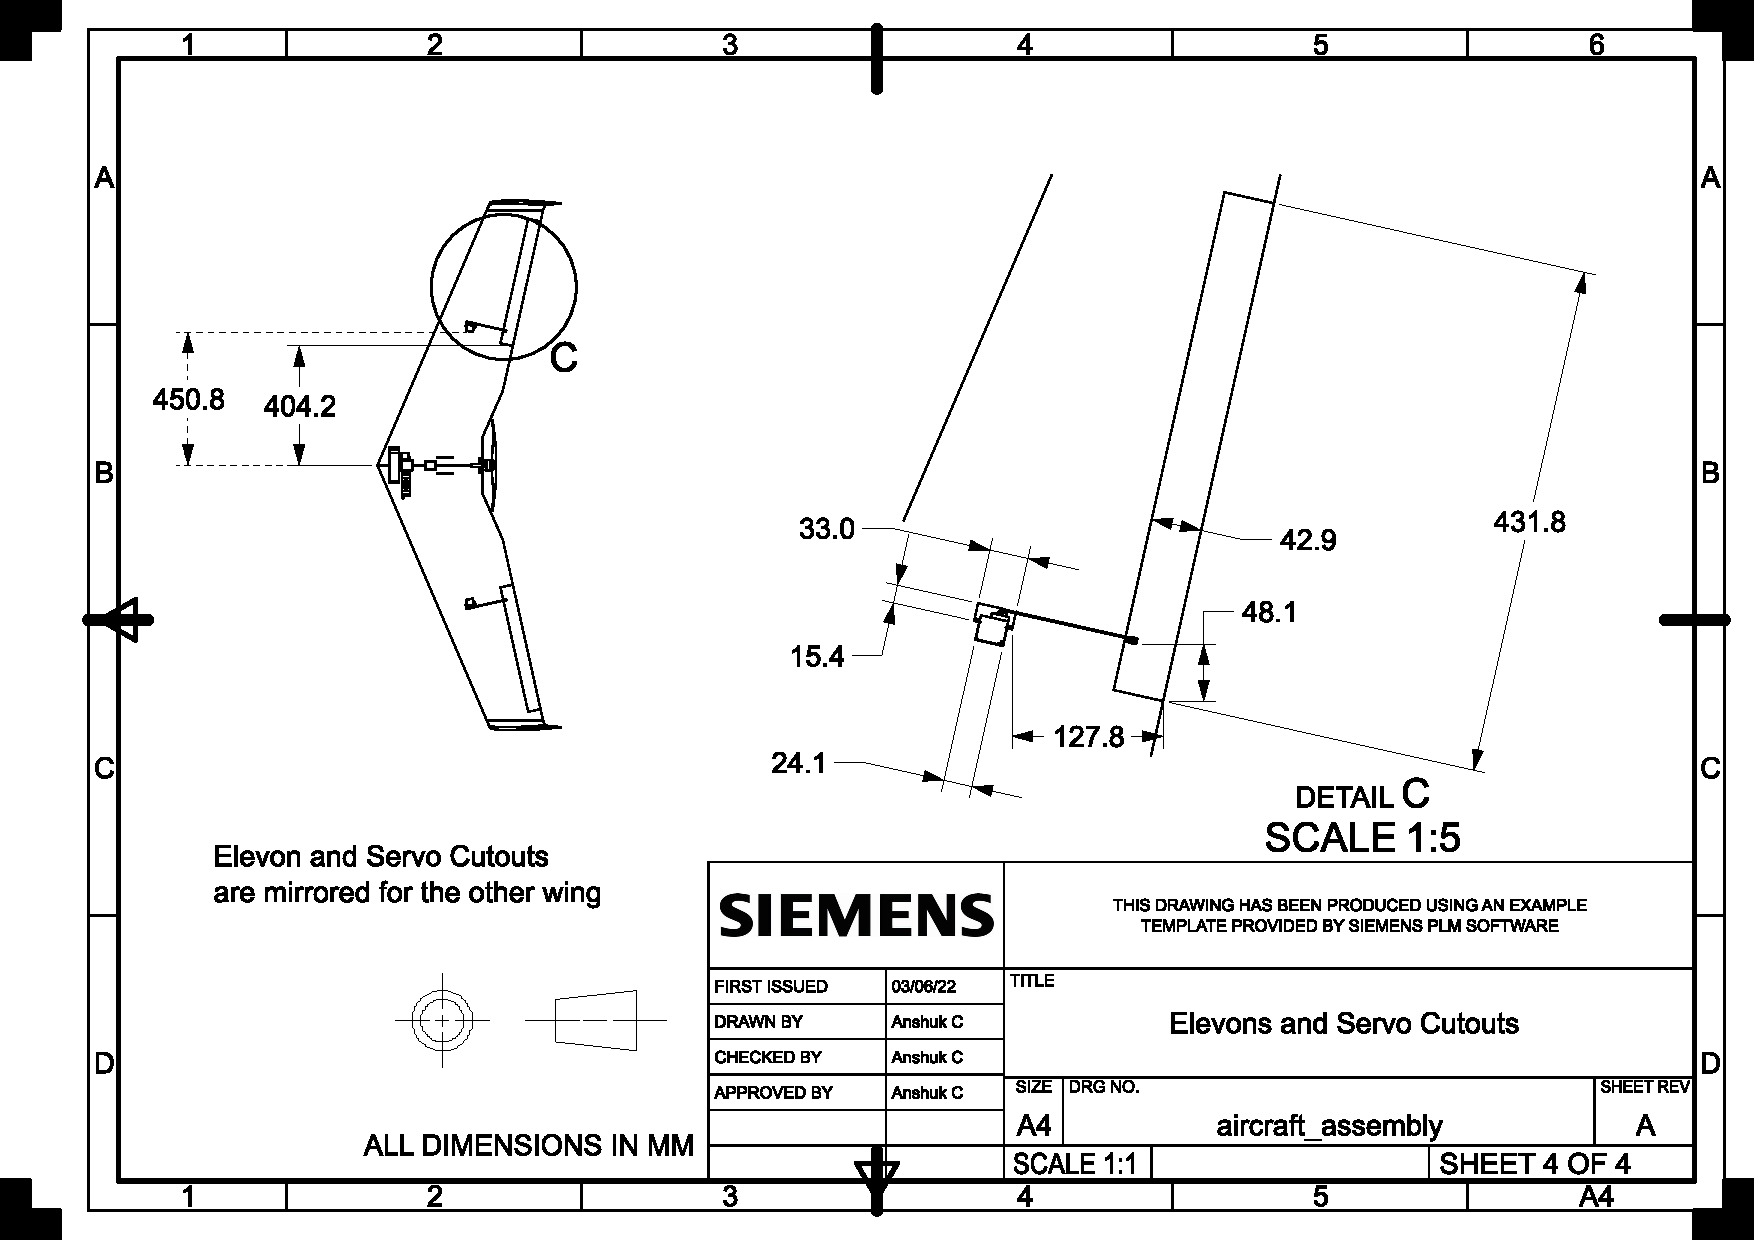
\includepdf[pages=-,angle=90]{homeworks/homework4/report/Figure/elevons_servos.pdf}
    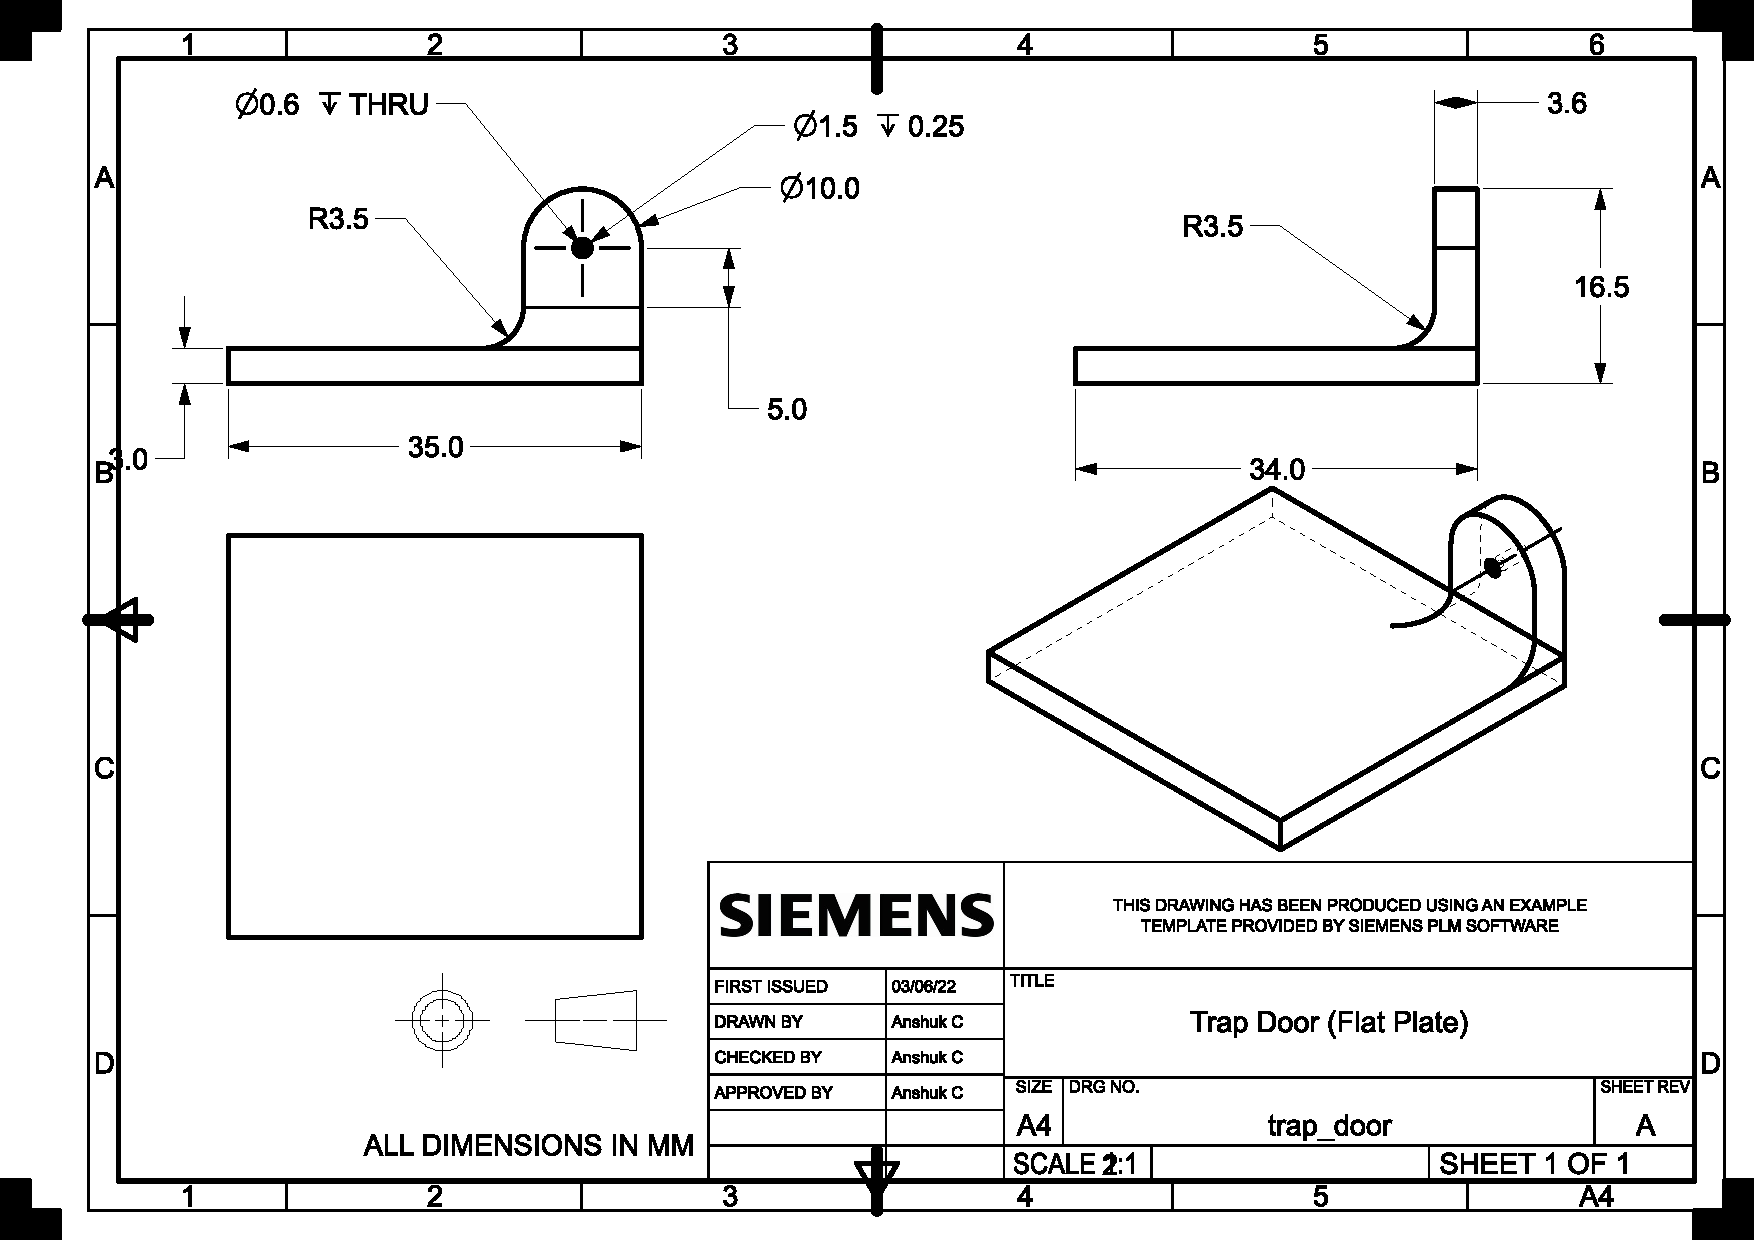
\includepdf[pages=-,angle=90]{homeworks/homework4/report/Figure/vial_plate_drawing.pdf}
    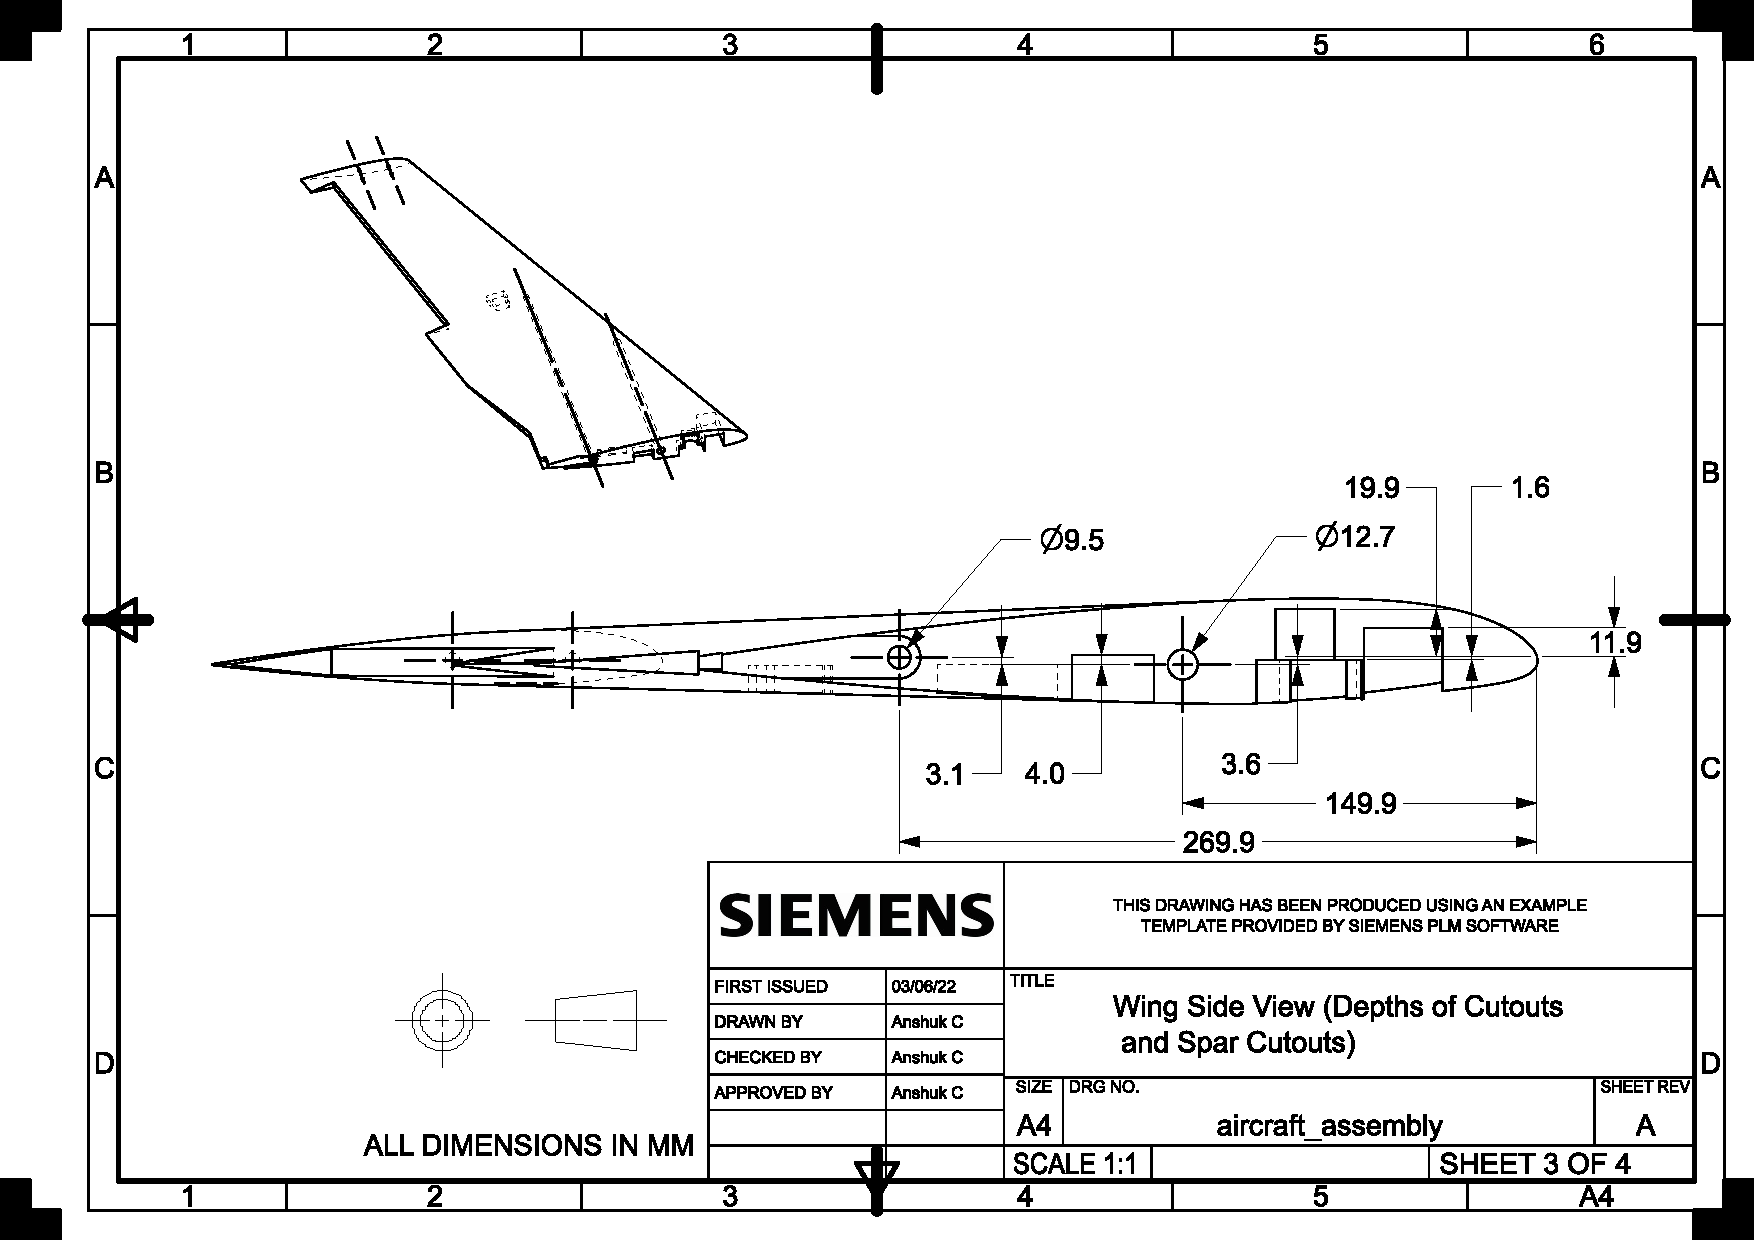
\includepdf[pages=-,angle=90]{homeworks/homework4/report/Figure/wing_depths_spar_cutouts.pdf}
    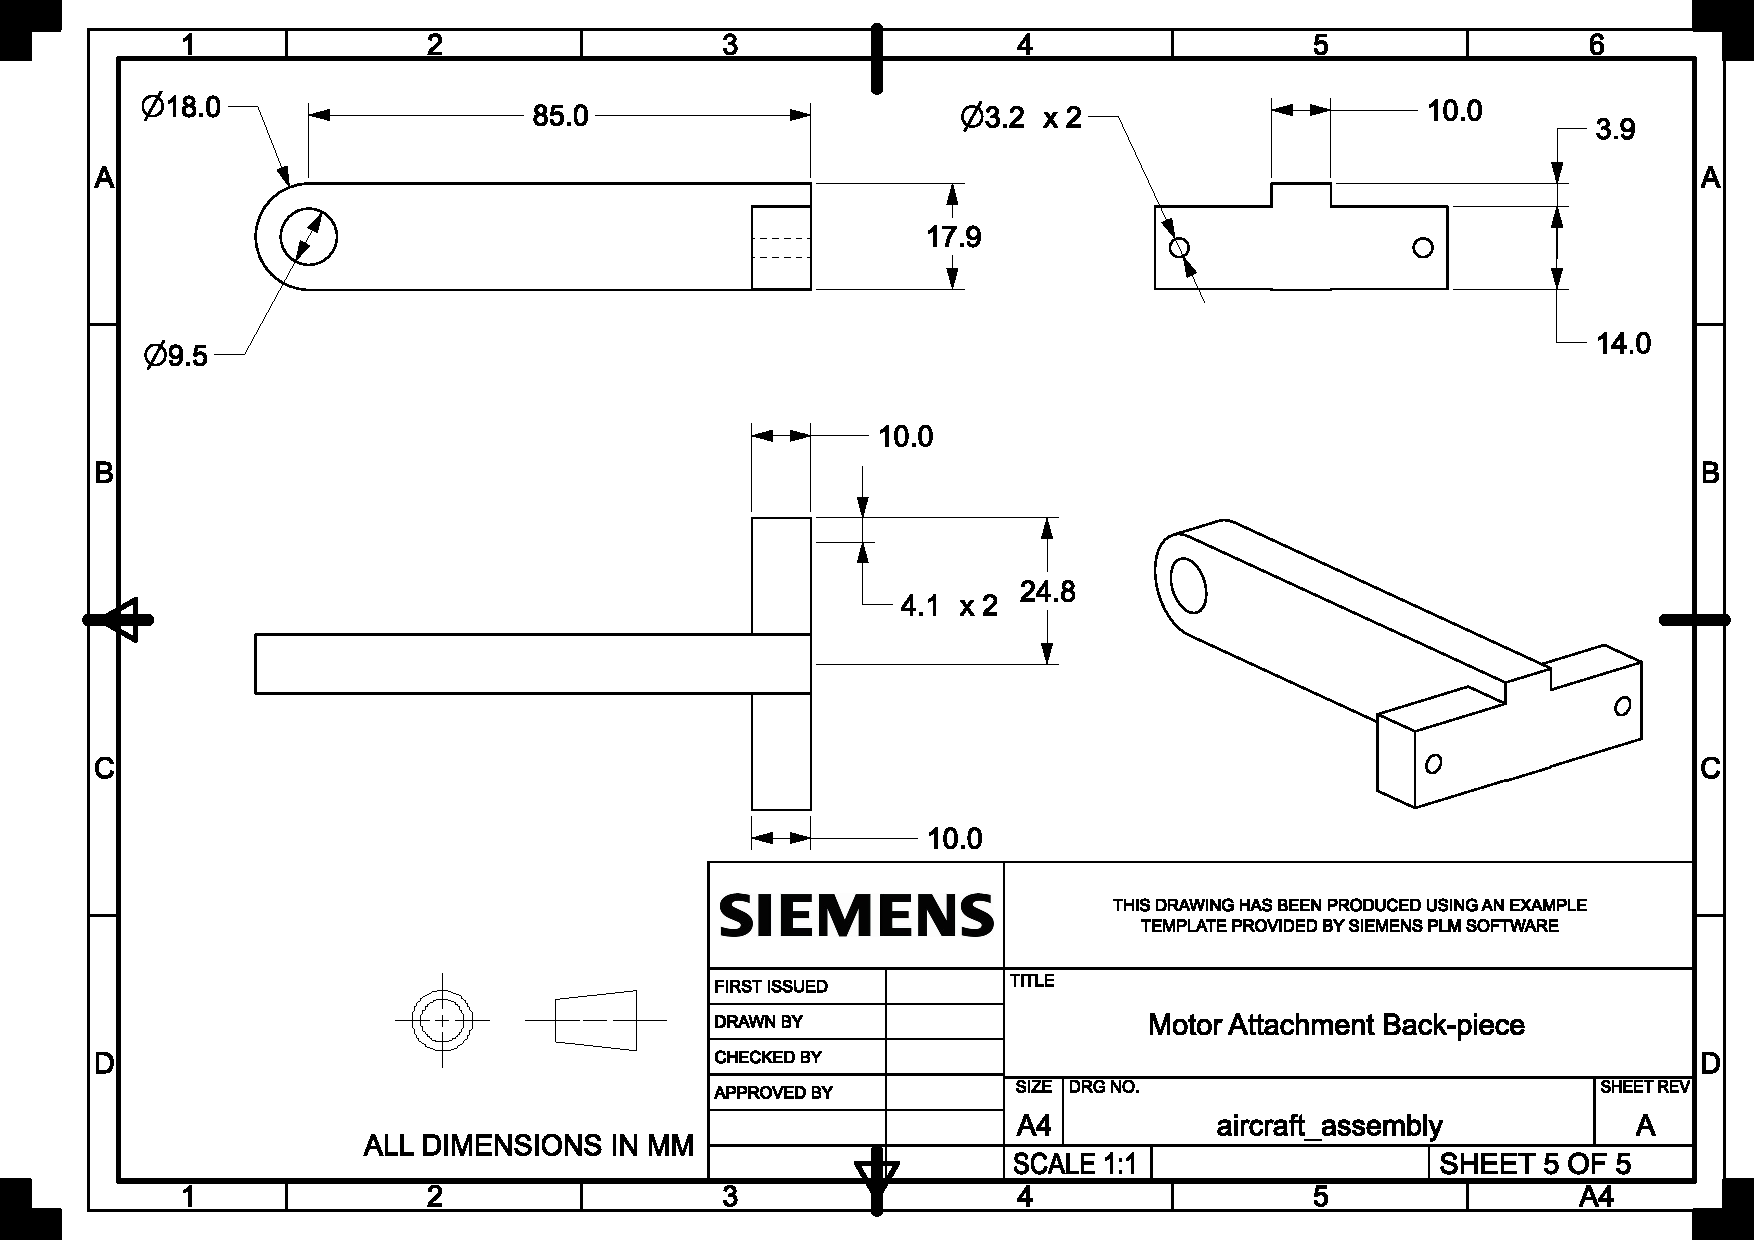
\includepdf[pages=-,angle=90]{homeworks/homework4/report/Figure/motor_holder.pdf}
    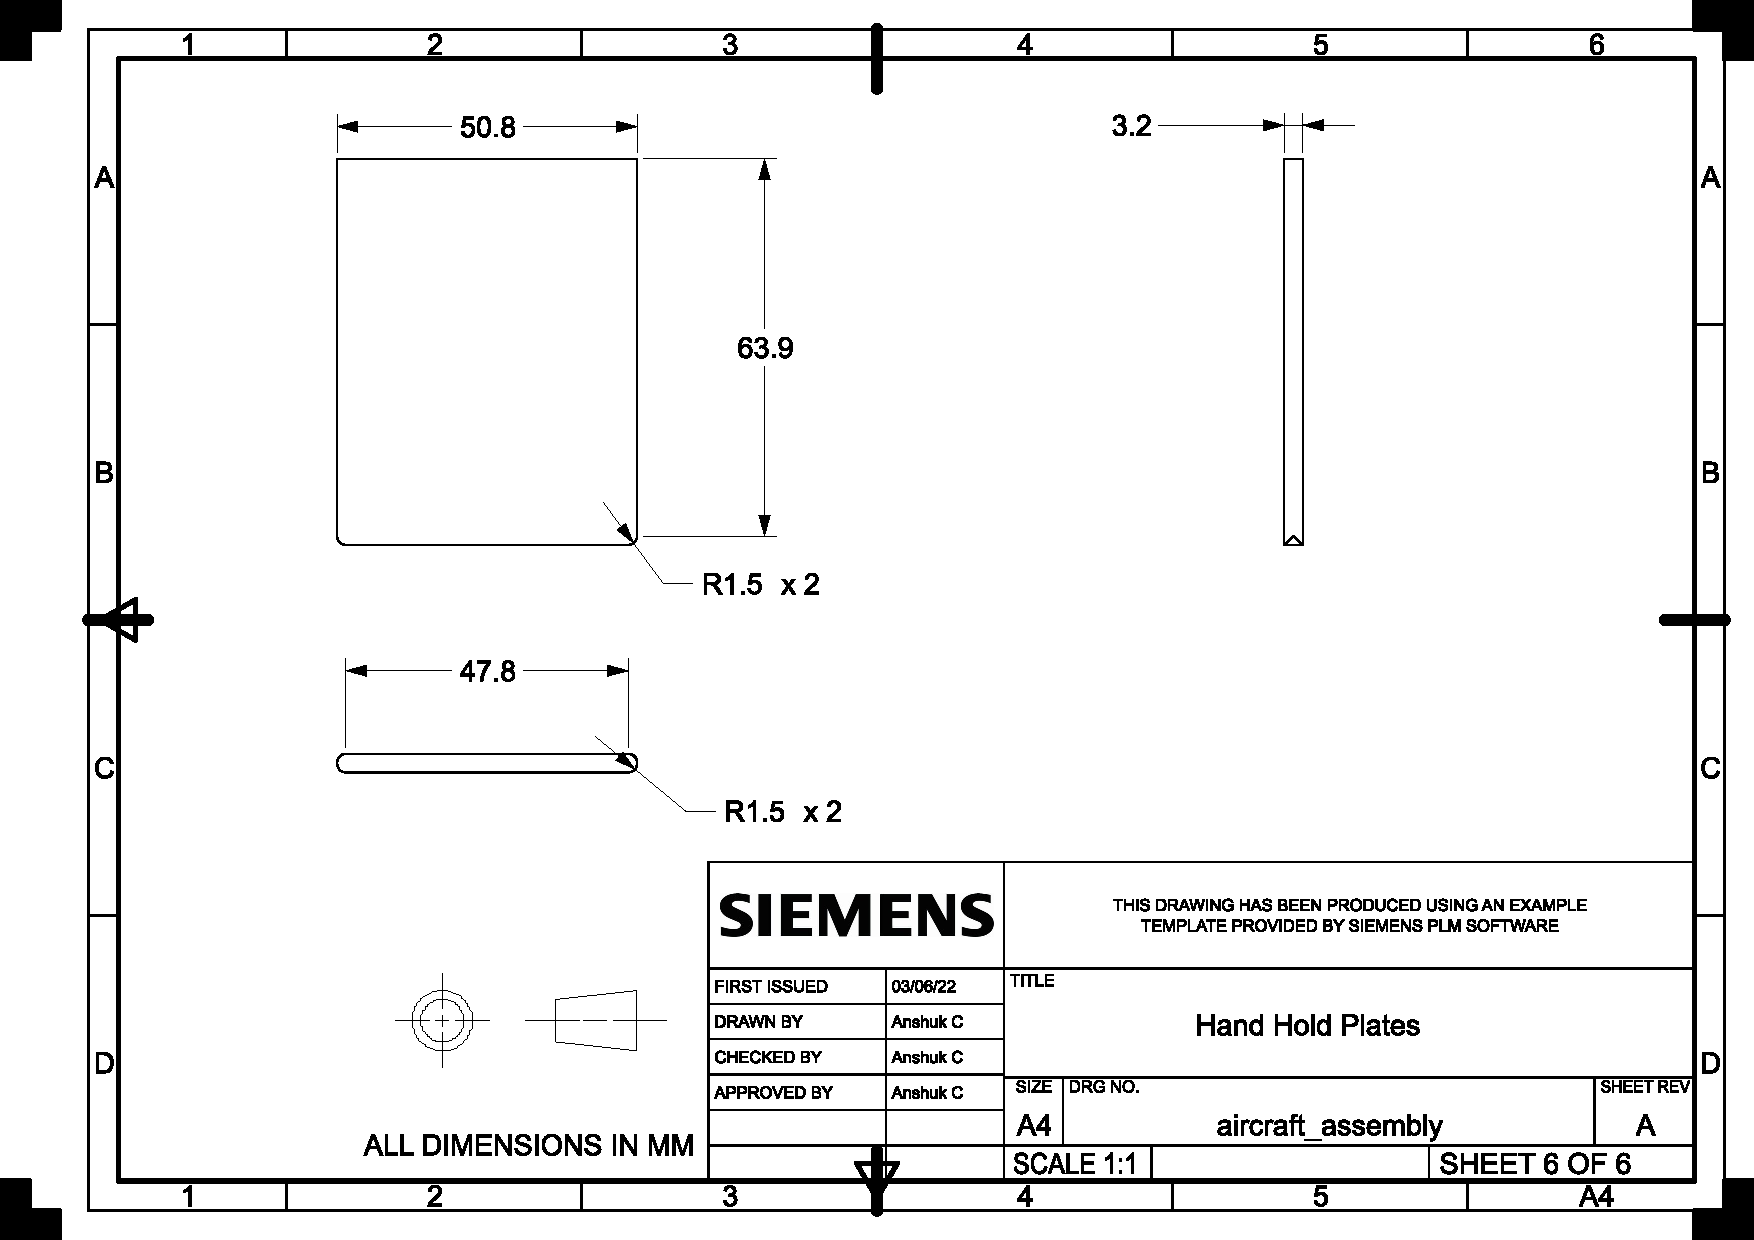
\includepdf[pages=-,angle=90]{homeworks/homework4/report/Figure/hand_holds.pdf}
    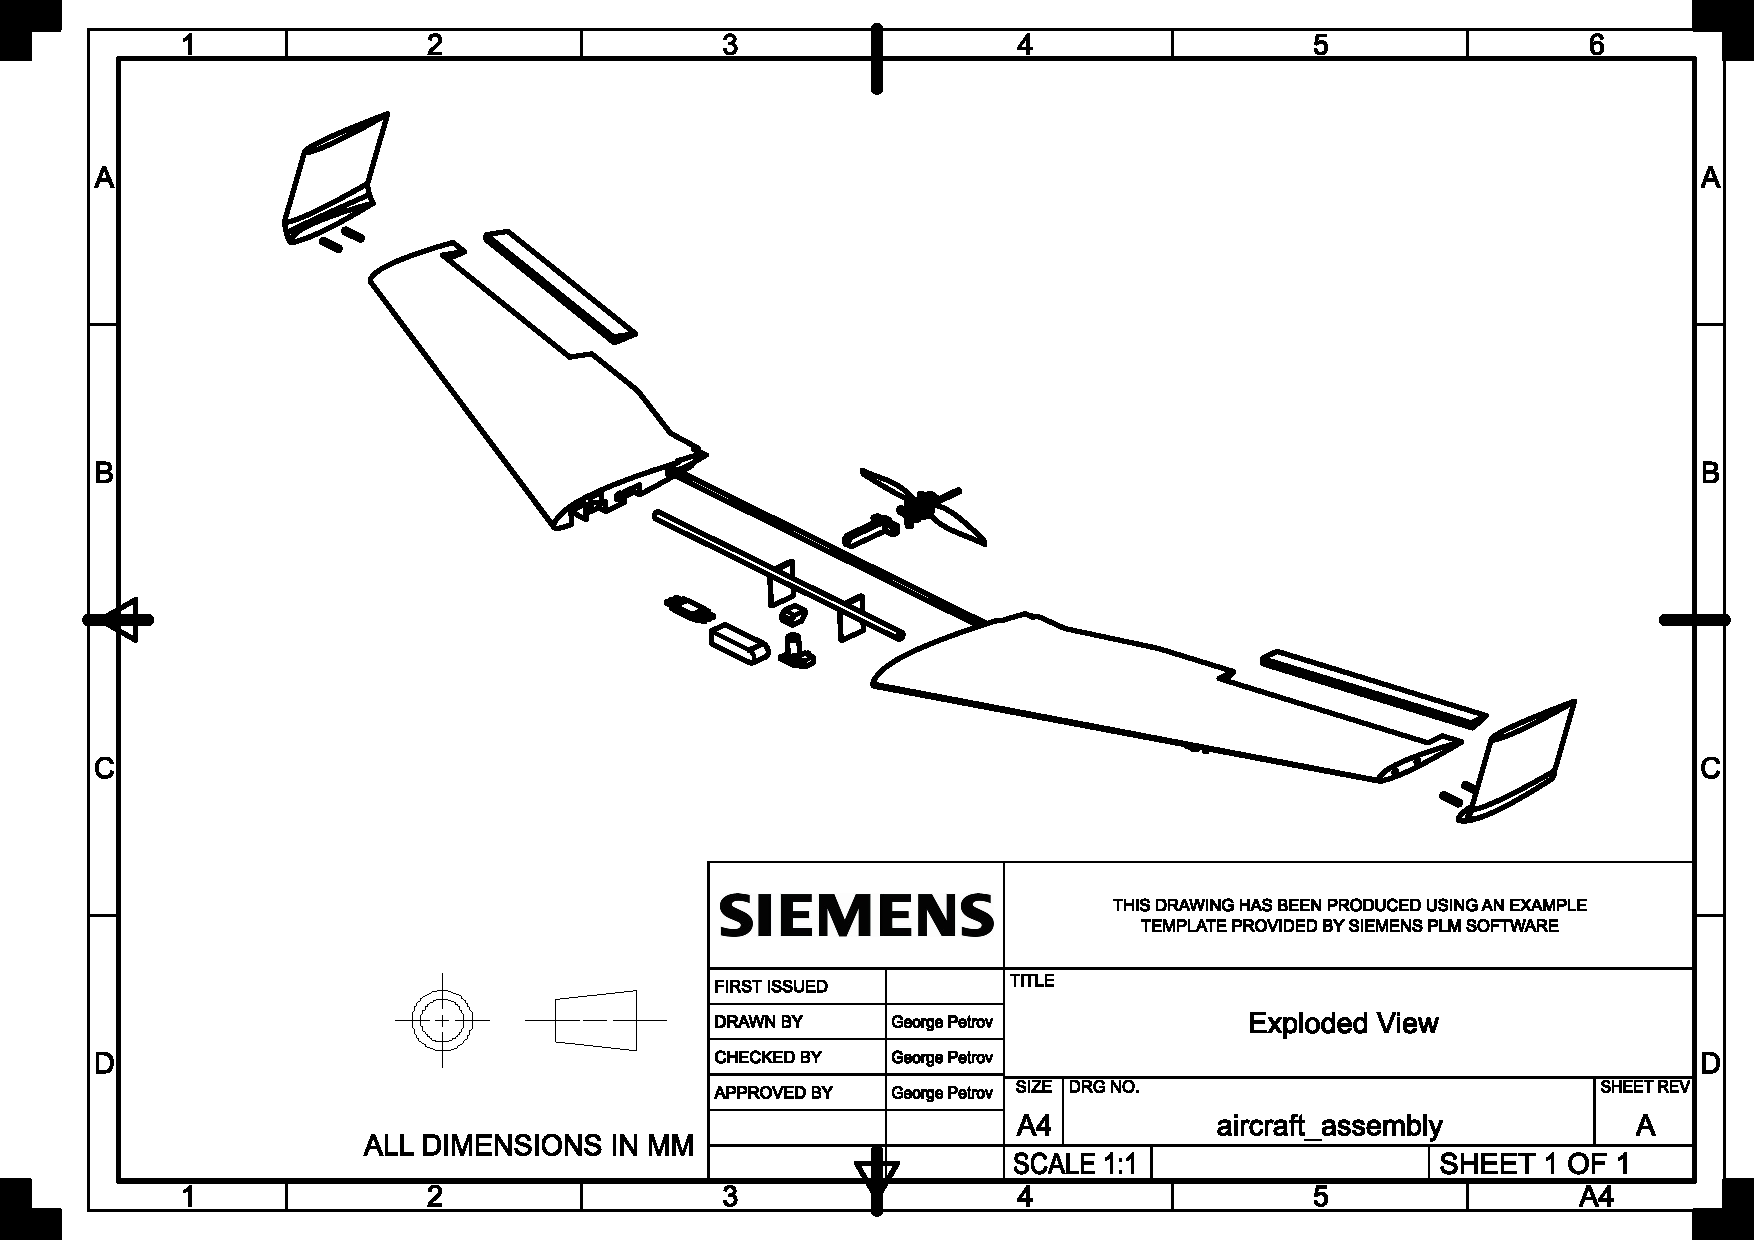
\includepdf[pages=-,angle=90]{homeworks/homework4/report/Figure/gpetrov2_aircraft_assembly_exploded_drawing.pdf}
    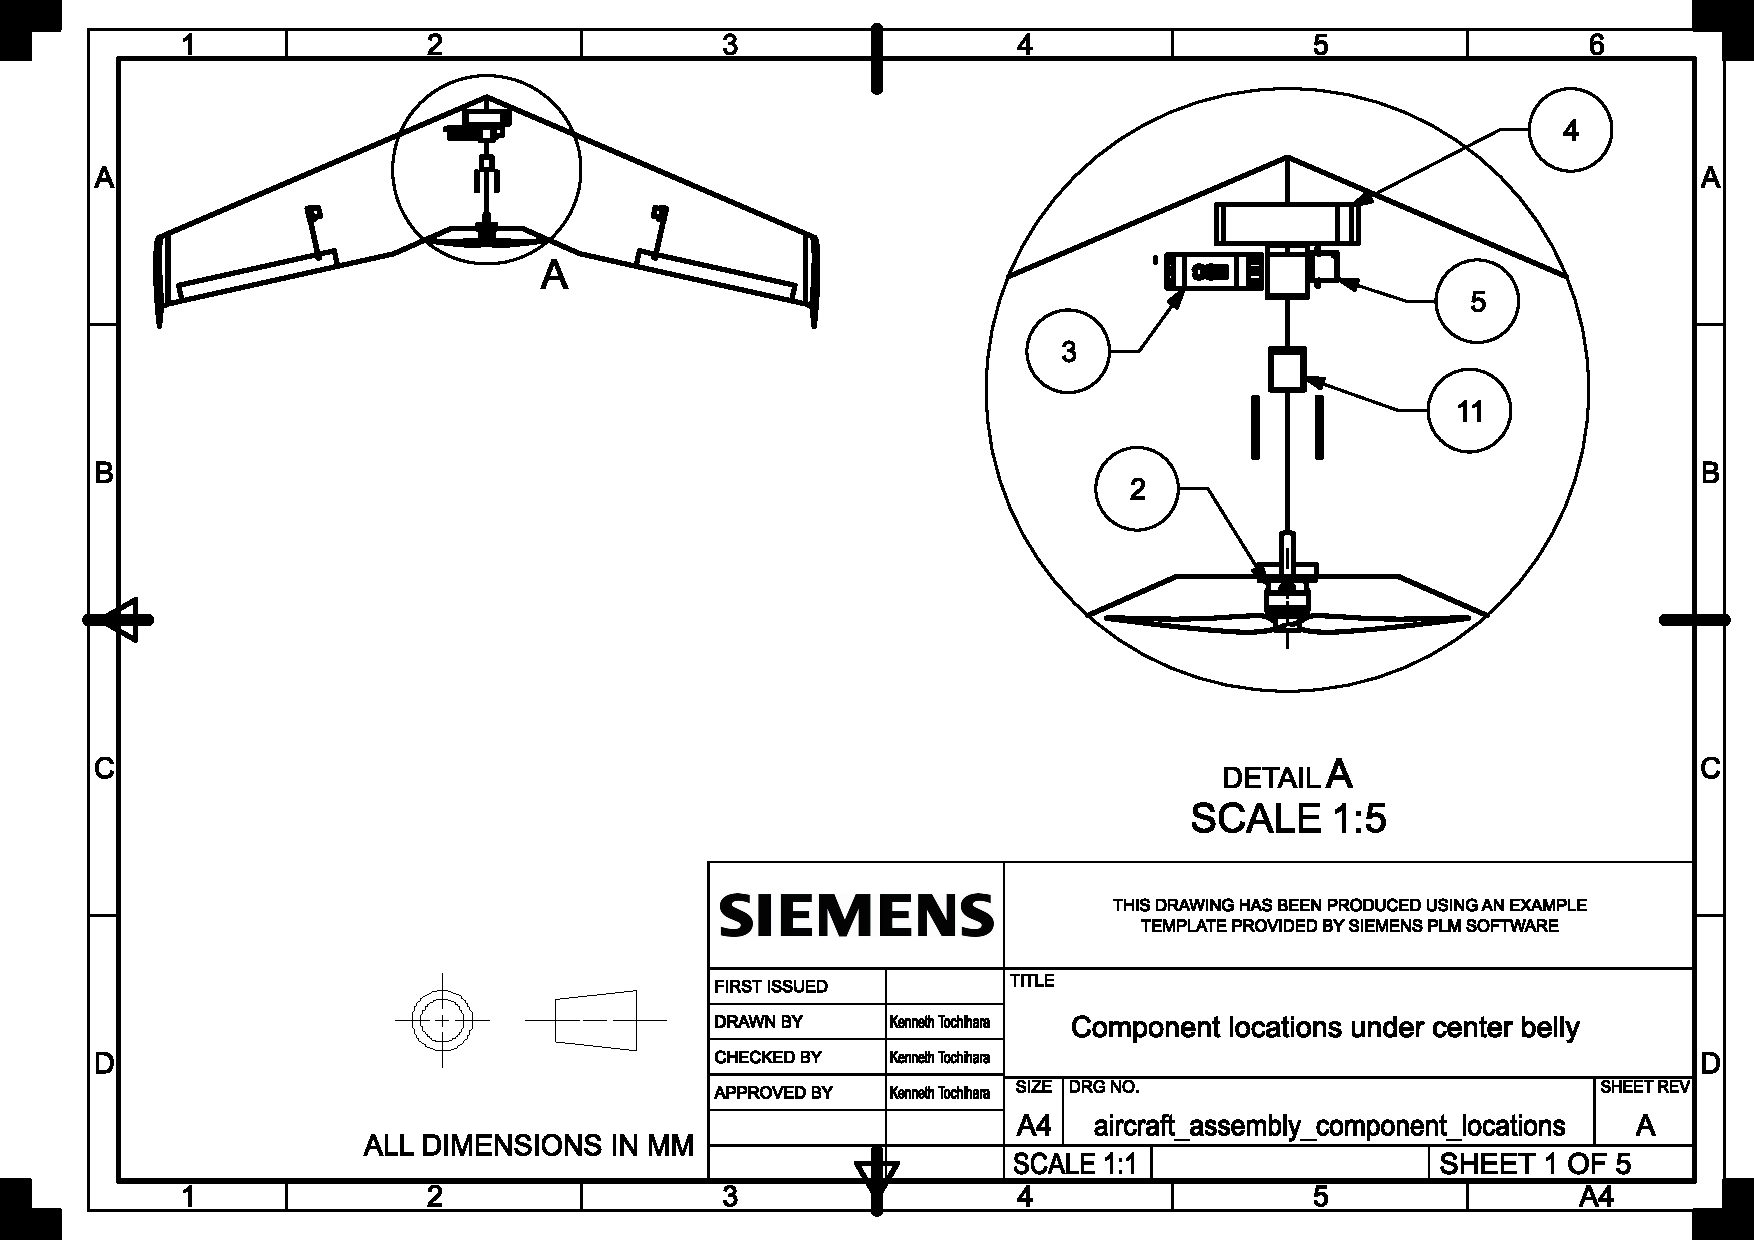
\includepdf[pages=-,angle=90]{homeworks/homework4/report/Figure/ktt3_aircraft_assembly_component_locations.pdf}


\section{Group Member Contributions} \label{apx:contributions}
% Make a table indicating how each group member contributed to the report

    \begin{table}[H]
        \begin{center} 
        \caption{\textbf{Group Member Contributions}}
        \begin{tabular}{ | p{2in} | p{4in}| } 
            \hline
            \textbf{Group Member} & \textbf{Contribution} \\  \hline
            Anshuk Chigullapalli & Designed vial release mechanism, assisted with cutouts, generated engineering drawings for fabricated components and full assembly\\ \hline
            Max Kaiser & Created the XFLR5 model of the UAV, with and without winglets. Completed sections 5,6 and 7 of the report. \\ \hline
            George Petrov & Designed wing, designed cutouts, integrated components, generated exploded views, sample calculations \\ \hline
            Kenneth Tochihara & Designed elevon actuator, designed cutouts, integrated components, generated equipment locations, managed repository \\ \hline
            Jeffery Zhou & Completed sections 3 and 4 of the report\\ \hline
        \end{tabular}
        \end{center}
    \end{table}
    
\end{enumerate}